\title{ TaxCalculator }
\author{Joe}
\date{\today}

\documentclass[12pt]{article}

\usepackage{tikz}
\usetikzlibrary{shapes,arrows}

\usepackage{listings}
\definecolor{mygreen}{rgb}{0,0.6,0}
\definecolor{mygray}{rgb}{0.5,0.5,0.5}
\definecolor{mymauve}{rgb}{0.58,0,0.82}

\usepackage{graphicx}
\graphicspath{ {./} }

\lstset{numbers=left,commentstyle=\color{mygreen},keywordstyle=\color{blue}}


\begin{document}
\maketitle
\pagebreak

% Source Code
% ===========

\section{Source Code}

Source code for \textsf{TaxCalculator.cs}
\lstinputlisting[language=c++,breaklines=true]{../TaxCalculator.cs}

\newpage

\lstinputlisting[breaklines=true]{../output.txt}

\newpage

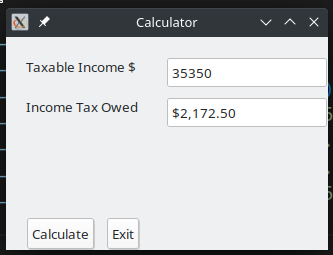
\includegraphics{Ex1}

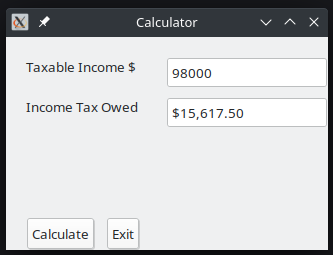
\includegraphics{Ex2}

\newpage

Autogenerated using scripts by Joe and \LaTeX.

Please find the full source code and binaries included.

\end{document}
